\documentclass[12pt,a4paper]{article}
\usepackage[utf8]{inputenc}
\usepackage[russian]{babel}
\usepackage{amsmath}
\usepackage{amssymb}
\usepackage{graphicx}
\usepackage{hyperref}
\usepackage{geometry}
\geometry{margin=1in}

\title{Лабораторная №2}
\author{Ануфриев Андрей}
\date{14.12.25}

\begin{document}

\maketitle

\section{Аналитическое описание множеств}

\subsection{Исходная область}

Исходная область $\Omega_z$ задаётся в комплексной плоскости $z = x + iy$ условиями:
\begin{equation}
\Omega_z = \{z = x + iy \mid x > 0,\, 0 < y < \pi\}
\end{equation}

Это \textbf{открытая горизонтальная полоса} шириной $\pi$ с левой границей на мнимой оси.

\subsection{Целевая область}

Целевая область $\Omega_w$ задаётся в комплексной плоскости $w = u + iv$ условиями:
\begin{equation}
\Omega_w = \{w = u + iv \mid v > 0,\, |w - i| > 1,\, |w + i| > 1\}
\end{equation}

Это \textbf{верхняя полуплоскость} со следующими исключениями:
\begin{itemize}
    \item Замкнутая единичная окружность с центром в точке $i$ и радиусом $1$: $|w - i| \leq 1$.
    \item Замкнутая единичная окружность с центром в точке $-i$ и радиусом $1$: $|w + i| \leq 1$.
\end{itemize}

Обе окружности полностью исключены из области.

\section{Композиция конформных отображений}

Построим последовательность отображений, переводящих $\Omega_z$ в $\Omega_w$.

\subsection{Шаг 1: Экспоненциальное отображение (№16 таблицы)}

\textbf{Отображение:}
\begin{equation}
\zeta = e^z, \quad z = \ln \zeta
\end{equation}

\textbf{Область определения:} $\zeta$-плоскость с $\operatorname{Im} \zeta > 0$ (верхняя полуплоскость).

\textbf{Свойства:}
\begin{itemize}
    \item Экспонента преобразует горизонтальную полосу $0 < \operatorname{Im} z < \pi$ в сектор с раствором $\pi$.
    \item При $z = x + iy$ с $0 < y < \pi$ имеем:
    \[
    \zeta = e^{x+iy} = e^x(\cos y + i \sin y)
    \]
    \item При $x \to 0^+$ получаем $|\zeta| \to 1$, при $x \to +\infty$ получаем $|\zeta| \to +\infty$.
    \item Вертикали $x = \text{const}$ переходят в окружности $|\zeta| = e^x$.
    \item Горизонтали $y = \text{const}$ переходят в лучи $\arg \zeta = y$.
    \item Левая граница $x = 0$ переходит в единичную окружность $|\zeta| = 1$.
\end{itemize}

\textbf{Проверка конформности:}
\[
\frac{d\zeta}{dz} = e^z \neq 0 \quad \forall z \in \Omega_z
\]

\subsection{Шаг 2: Инверсия (№14 таблицы)}

\textbf{Отображение:}
\begin{equation}
\eta = \frac{1}{\zeta}, \quad \zeta = \frac{1}{\eta}
\end{equation}

\textbf{Область определения:} $\eta$-плоскость с $|\eta| < 1$ (открытый единичный круг).

\textbf{Свойства:}
\begin{itemize}
    \item Инверсия переводит внешность единичного круга во внутренность.
    \item Верхняя полуплоскость переходит во внутренность единичного круга.
    \item Окружность $|\zeta| = 1$ остаётся на месте.
    \item Окружность $|\zeta| = e^x$ (при $x > 0$) переходит в окружность $|\eta| = e^{-x}$ (радиус убывает).
\end{itemize}

\textbf{Проверка конформности:}
\[
\frac{d\eta}{d\zeta} = -\frac{1}{\zeta^2} \neq 0 \quad \forall \zeta \neq 0
\]

\subsection{Шаг 3: отображение Жуковского (№30/31 таблицы)}

\textbf{Отображение:}
\begin{equation}
w = \frac{1}{2}\left(\eta + \frac{1}{\eta}\right),
\qquad
\eta = \eta(w) \text{ — одна из ветвей решения уравнения } \eta^2 - 2w\eta + 1 = 0.
\end{equation}

\textbf{Область определения:} единичный круг
\begin{equation}
\Omega_\eta = {\eta = s + it \mid |\eta| < 1}.
\end{equation}

\textbf{Образ:} верхняя полуплоскость с вырезанными единичными кругами вокруг точек 
±
1
±1:
\begin{equation}
\Omega_w = {w = u + iv \mid v > 0,\ |w - 1| > 1,\ |w + 1| > 1}.
\end{equation}

\textbf{Свойства:}
\begin{itemize}
\item При 
∣
η
∣
<
1
∣η∣<1 точка 
η
η лежит внутри единичного круга, а её образ 
w
w лежит в верхней полуплоскости вне двух единичных кругов 
∣
w
−
1
∣
≤
1
∣w−1∣≤1 и 
∣
w
+
1
∣
≤
1
∣w+1∣≤1.
\item Граница единичного круга 
∣
η
∣
=
1
∣η∣=1 отображается в отрезок 
[
−
1
,
1
]
[−1,1] на вещественной оси:
η
=
e
i
φ
,
 
∣
η
∣
=
1
  
⇒
  
w
=
1
2
(
e
i
φ
+
e
−
i
φ
)
=
cos
⁡
φ
∈
[
−
1
,
1
]
.
η=e 
iφ
 , ∣η∣=1⇒w= 
2
1
 (e 
iφ
 +e 
−iφ
 )=cosφ∈[−1,1].
\item Окружности 
∣
η
∣
=
r
<
1
∣η∣=r<1 переходят в замкнутые кривые в 
w
w-плоскости (эллипсы), которые огибают вырезанные единичные круги с центрами в точках 
w
=
±
1
w=±1.
\item Таким образом, после шага 3 единичный круг 
Ω
η
Ω 
η
  превращается в область 
Ω
w
Ω 
w
 , представляющую собой всю верхнюю полуплоскость, кроме двух единичных полусфер (верхних полукругов) с центрами в точках 
(
−
1
,
0
)
(−1,0) и 
(
1
,
0
)
(1,0).
\end{itemize}

\textbf{Проверка конформности:}
\begin{equation}
\frac{dw}{d\eta} = \frac{1}{2}\left(1 - \frac{1}{\eta^2}\right).
\end{equation}
\section{Итоговое отображение}

Композиция трёх шагов дает явную формулу:
\begin{equation}
w(z) = \frac{1}{2}\left(e^{-z} + e^{z}\right) = \cosh z
\end{equation}

\textbf{Это отображение полосы $\Omega_z = \{0 < \operatorname{Im} z < \pi,\, \operatorname{Re} z > 0\}$ в область $\Omega_w$.}

\subsection{Проверка на границах}

При $z = x + iy$ где $x \geq 0$, $0 \leq y \leq \pi$:

\begin{itemize}
    \item \textbf{Граница $y = 0$:} $w = \cosh x = \frac{e^x + e^{-x}}{2}$ — вещественная полуось $[1, +\infty)$.
    
    \item \textbf{Граница $y = \pi$:} $w = \cosh(x + i\pi) = \cosh x \cos \pi - i \sinh x \sin \pi = -\cosh x$ — вещественная полуось $(-\infty, -1]$.
    
    \item \textbf{Граница $x = 0$:} $w = \cosh(iy) = \cos y$ — отрезок $[-1, 1]$ на вещественной оси.
\end{itemize}

\section{Обратное отображение}

Обратное отображение вычисляется стандартной формулой для гиперболического косинуса:
\begin{equation}
z(w) = \text{arcosh } w = \ln\bigl(w + \sqrt{w^2 - 1}\bigr)
\end{equation}

где ветвь логарифма выбирается так, чтобы $\operatorname{Im} z(w) \in (0, \pi)$.

\textbf{Проверка:}
\[
\frac{dz}{dw} = \frac{1}{\sqrt{w^2 - 1}} \neq 0 \quad \text{при } w \notin [-1, 1]
\]

Отображение $z(w)$ определено и конформно на всей области $\Omega_w$.

\section{Таблица отображений}

\begin{center}
\begin{tabular}{|c|c|c|c|}
\hline
\textbf{Шаг} & \textbf{Отображение} & \textbf{№ таблицы} & \textbf{Область} \\
\hline
$z \to \zeta$ & $\zeta = e^z$ & №16 & $\operatorname{Im} \zeta > 0$ \\
$\zeta \to \eta$ & $\eta = 1/\zeta$ & №14 & $|\eta| < 1$ \\
$\eta \to w$ & $w = \frac{1}{2}(\eta + 1/\eta)$ & №30/31 & $\operatorname{Im} w > 0$ \\
\hline
\textbf{Композиция} & $w = \cosh z$ & №52 & $\Omega_w$ \\
\hline
\end{tabular}
\end{center}

\section{Геометрическая интерпретация}

\subsection{Трансформация сетки}

\begin{itemize}
    \item \textbf{Вертикали полосы} ($x = \text{const}$) переходят через цепь преобразований в окружности вокруг $\pm i$.
    \item \textbf{Горизонтали полосы} ($y = \text{const}$) преобразуются в гиперболические кривые в целевой области.
    \item \textbf{Левая граница} ($x = 0$) переходит в отрезок $[-1, 1]$ на вещественной оси.
    \item \textbf{Нижняя граница} ($y = 0$) переходит в положительную полуось $[1, +\infty)$.
    \item \textbf{Верхняя граница} ($y = \pi$) переходит в отрицательную полуось $(-\infty, -1]$.
\end{itemize}

\subsection{Конформность}

Полная производная композиции:
\begin{equation}
\frac{dw}{dz} = \frac{dw}{d\eta} \cdot \frac{d\eta}{d\zeta} \cdot \frac{d\zeta}{dz} = \frac{1}{2}\left(1 - \frac{1}{\eta^2}\right) \cdot \left(-\frac{1}{\zeta^2}\right) \cdot e^z = \sinh z \neq 0
\end{equation}

Равносильно: $\frac{dw}{dz} = \sinh z = \frac{e^z - e^{-z}}{2}$.

Итак, отображение \textbf{конформно} везде в $\Omega_z$.

\section{Визуализация}

Программа \texttt{conformal\_cosh\_mapping.py} генерирует четыре графика:

\begin{enumerate}
    \item \textbf{График 1 (исходная область):} Полоса с сеткой вертикальных и горизонтальных линий.
    \begin{figure}
        \centering
        
\includegraphics[width=1\linewidth]{picture1.png}
        \caption{начальный график}
        \label{fig:placeholder}
    \end{figure}
    \item \textbf{График 2 (после шага 1):} Верхняя полуплоскость после применения $\zeta = e^z$.
    \begin{figure}
        \centering
        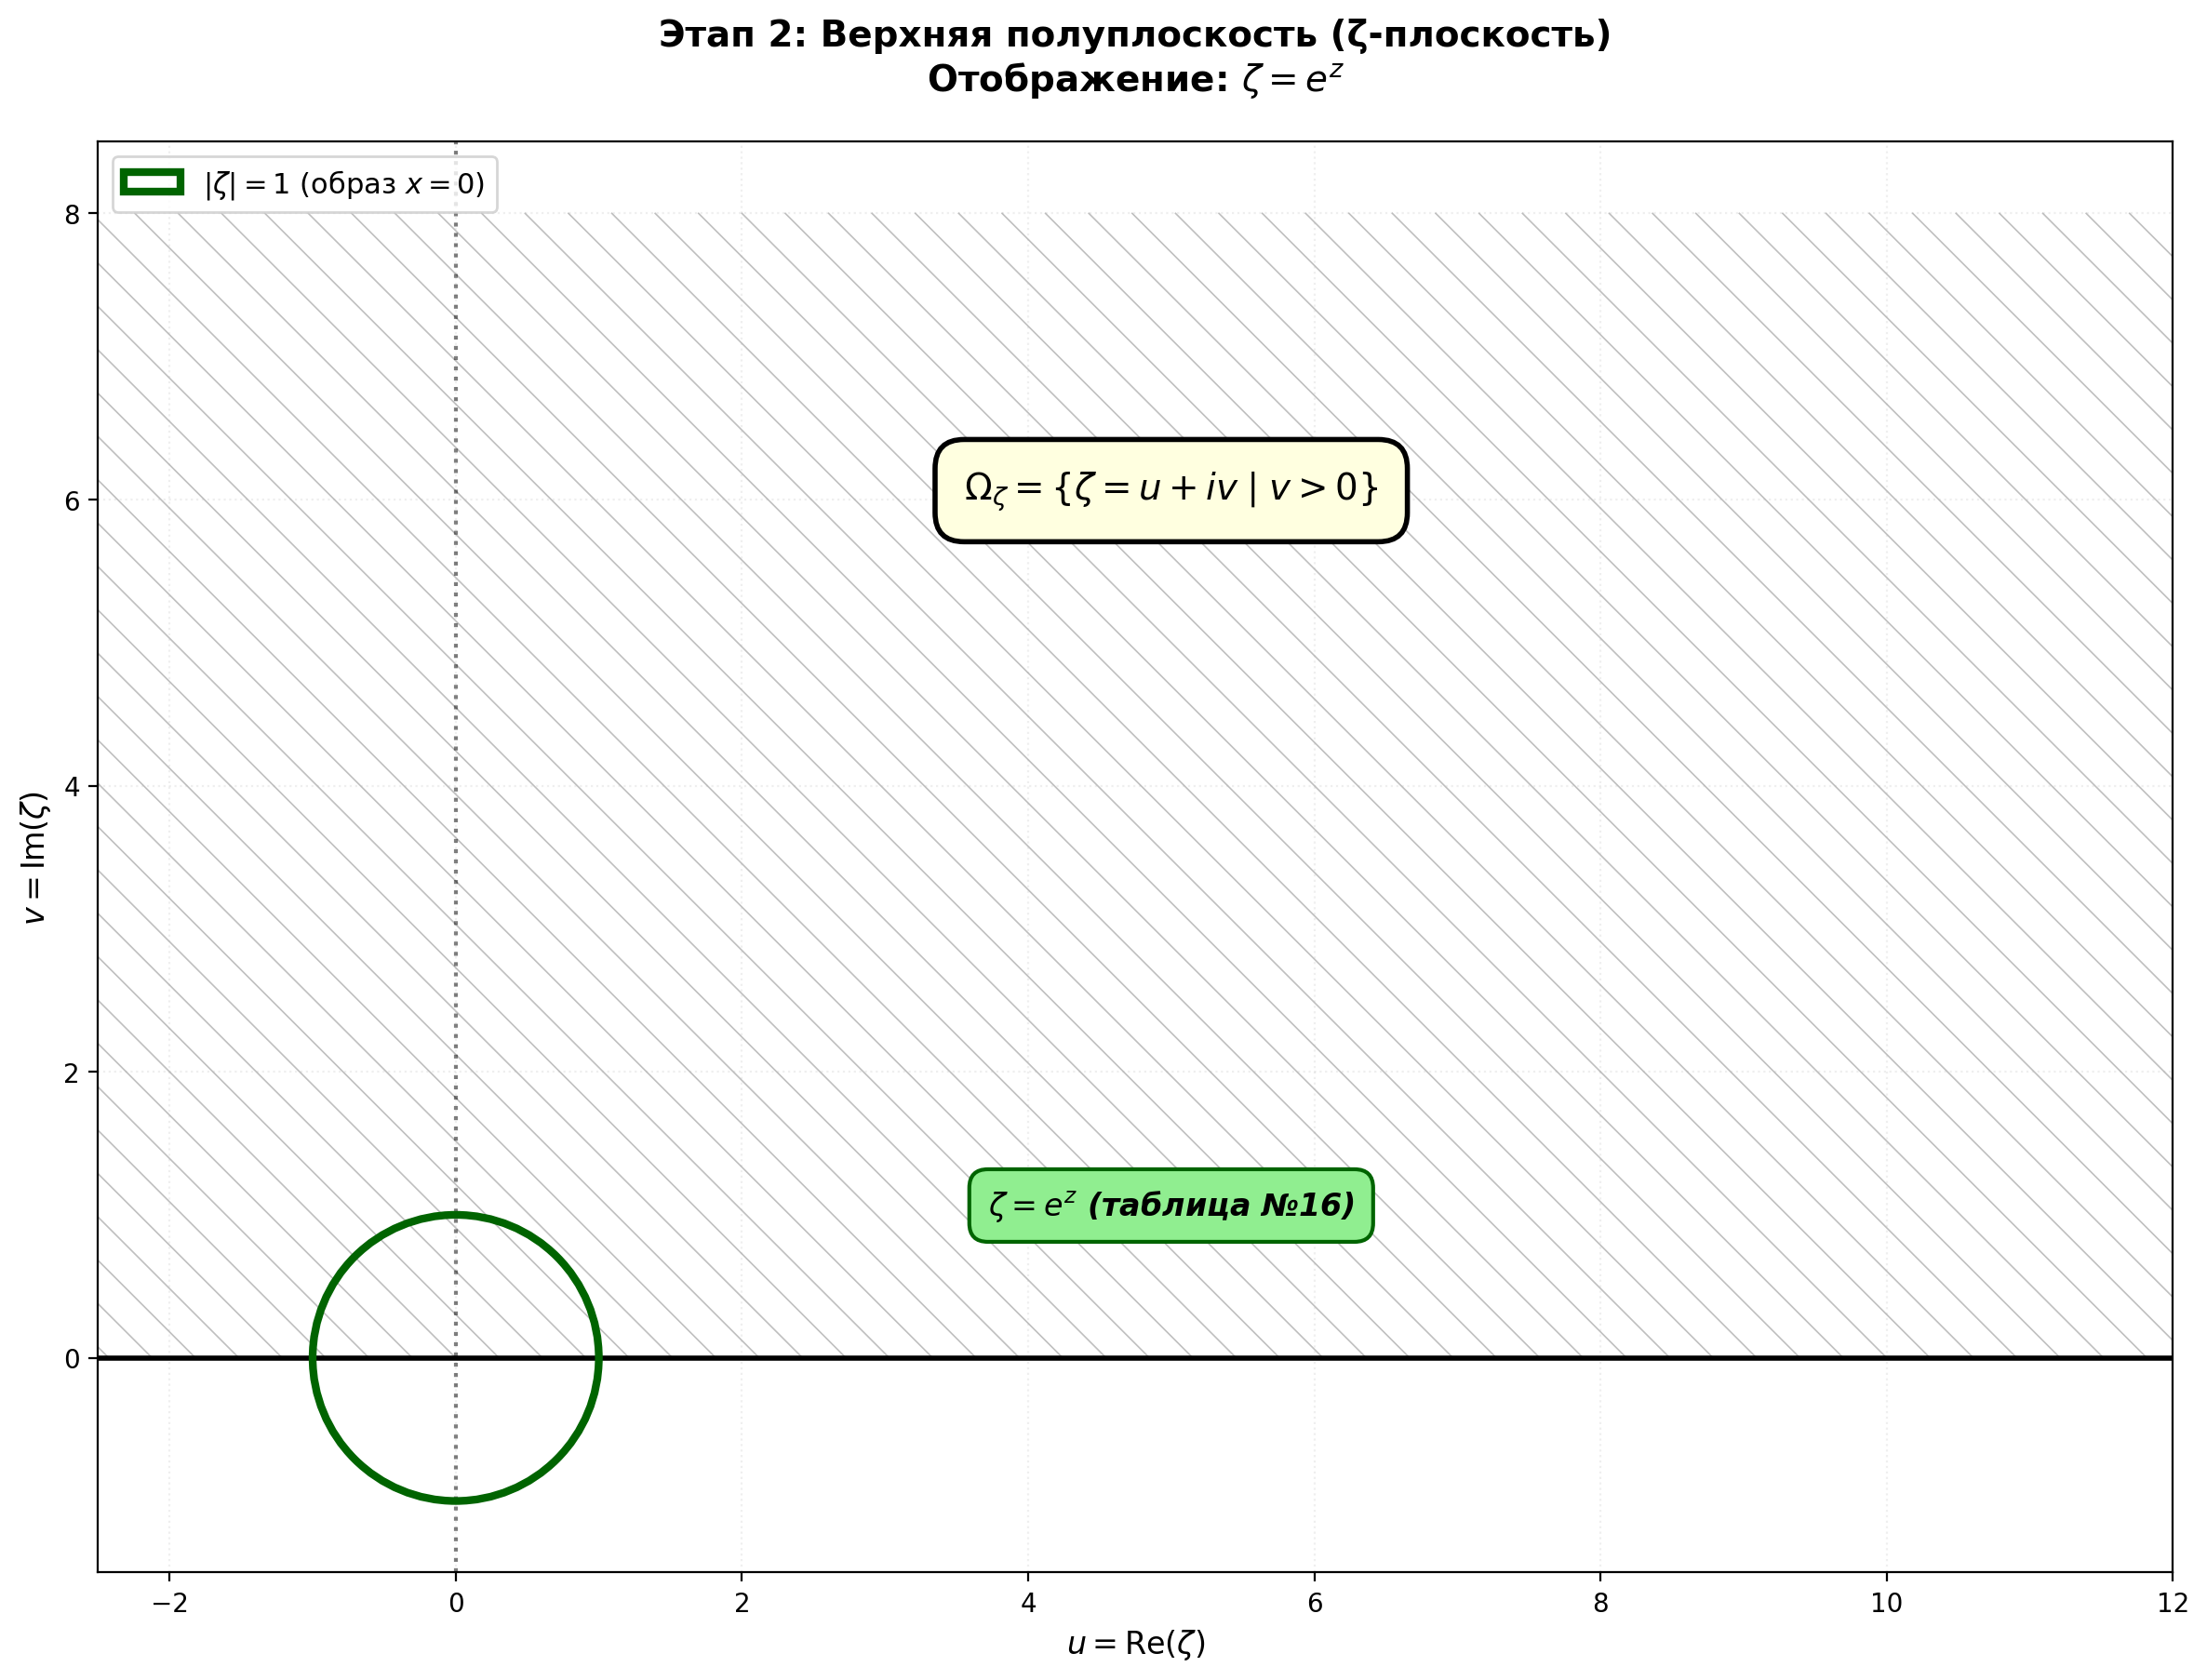
\includegraphics[width=1\linewidth]{image2.png}
        \caption{перевели в полусферу}
        \label{fig:placeholder}
    \end{figure}
    \item \textbf{График 3 (после шага 2):} Единичный круг после инверсии $\eta = 1/\zeta$.
    \begin{figure}
        \centering
        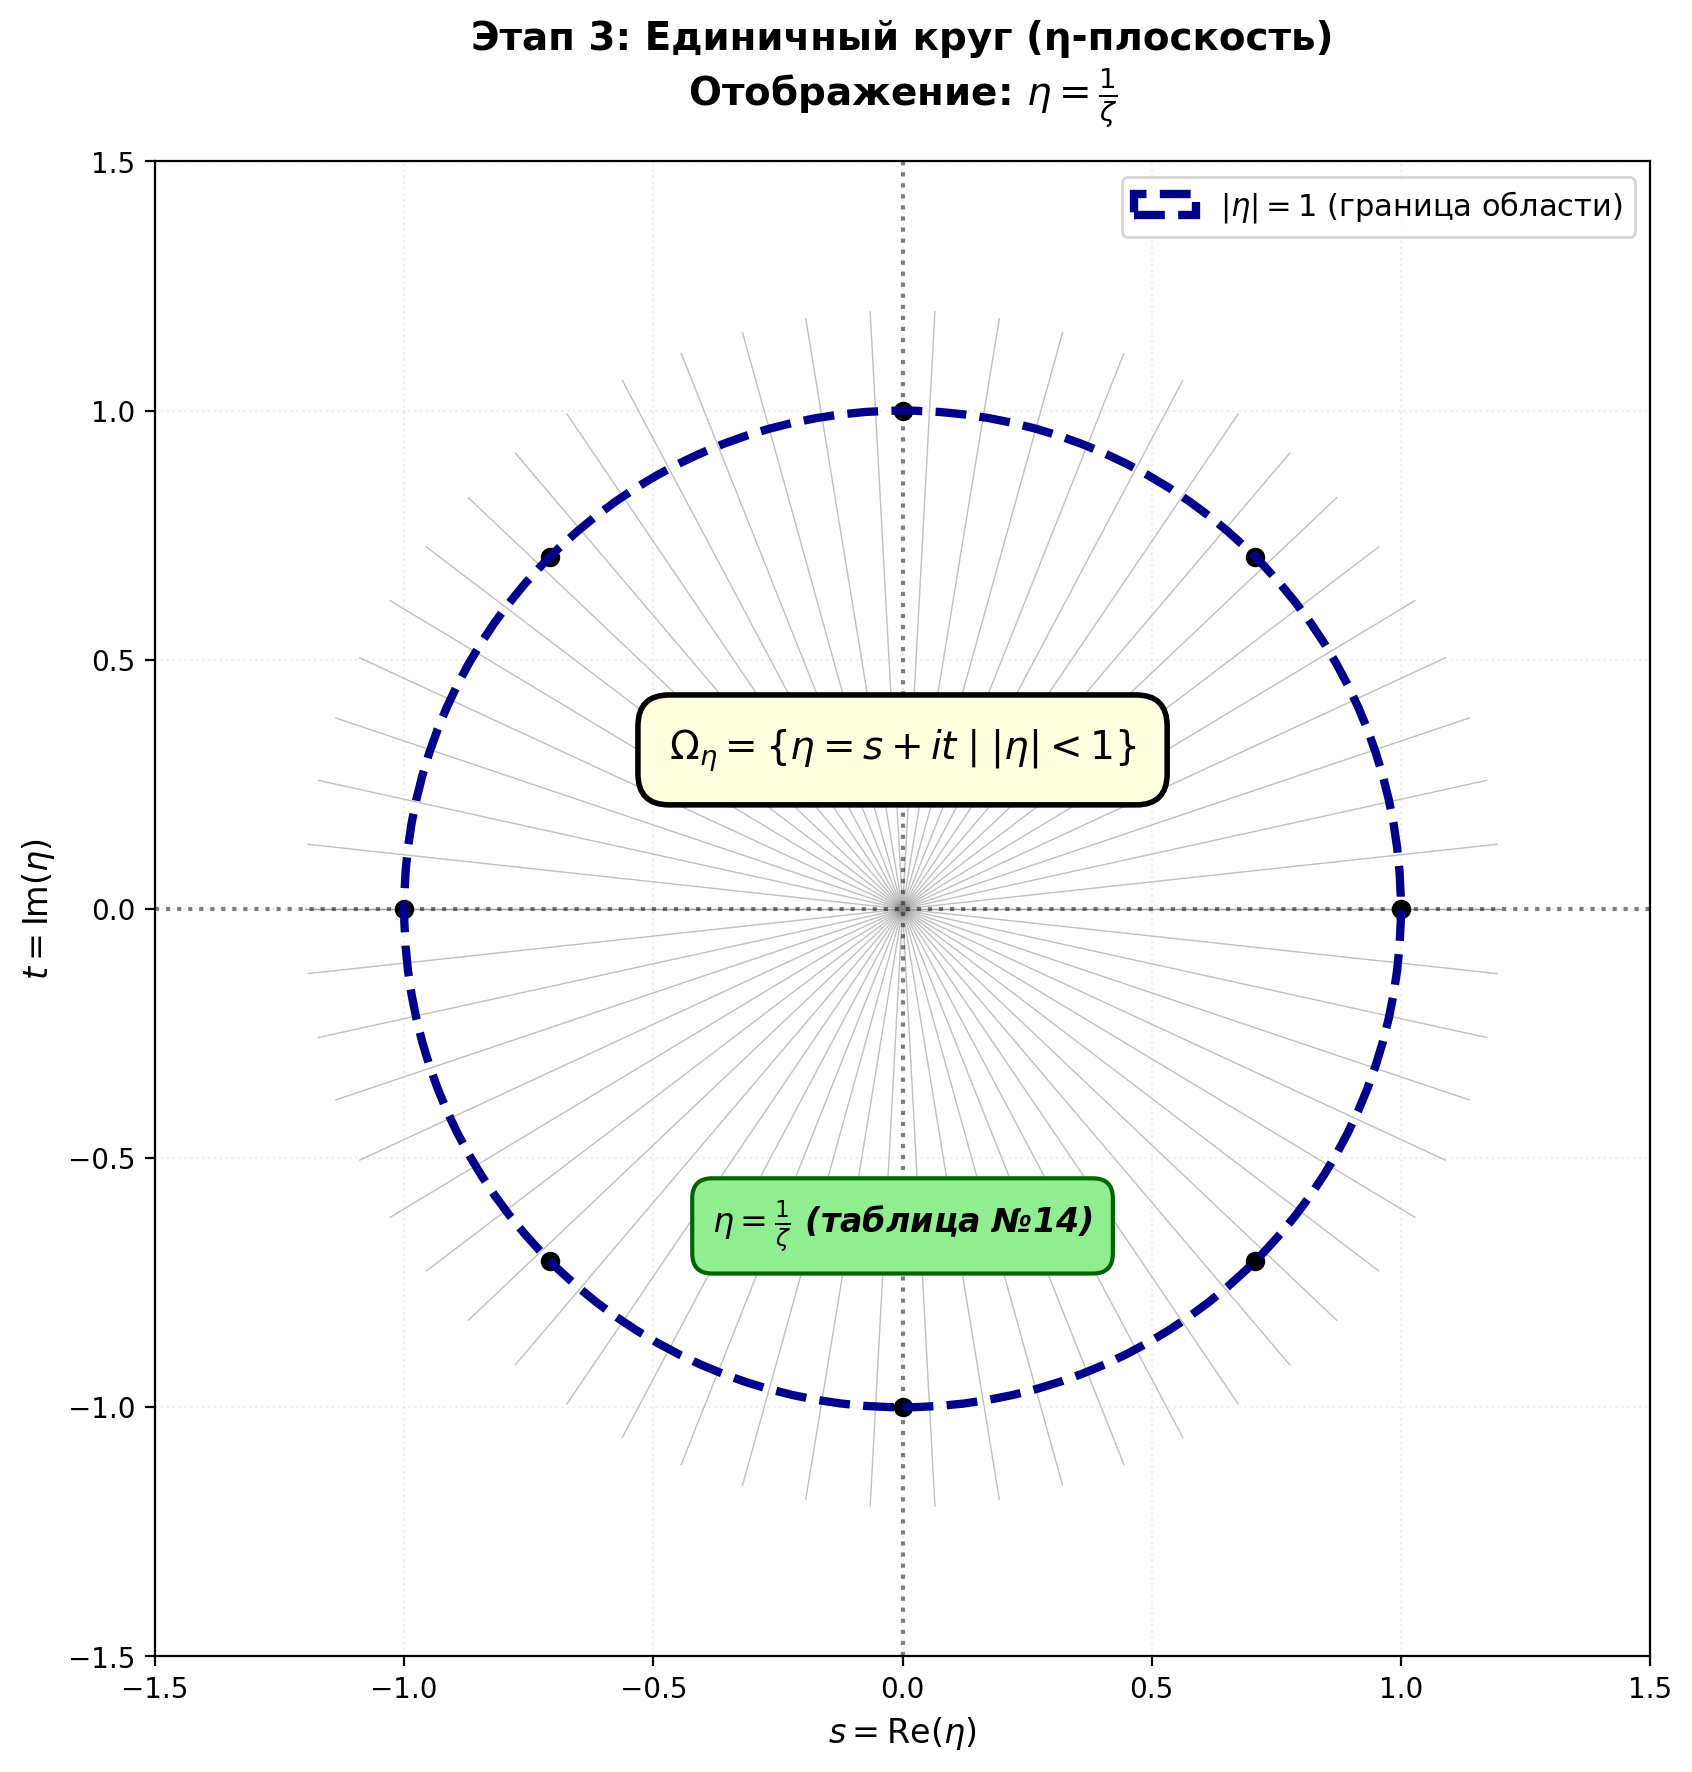
\includegraphics[width=1\linewidth]{image3.png}
        \caption{Взяли всё, кроме полусферы}
        \label{fig:placeholder}
    \end{figure}
    \item \textbf{График 4 (итоговая область):} Вер8Ыхняя полуплоскость с вырезанными окружностями после применения $w = \frac{1}{2}(\eta + 1/\eta)$.
\begin{figure}
    \centering
    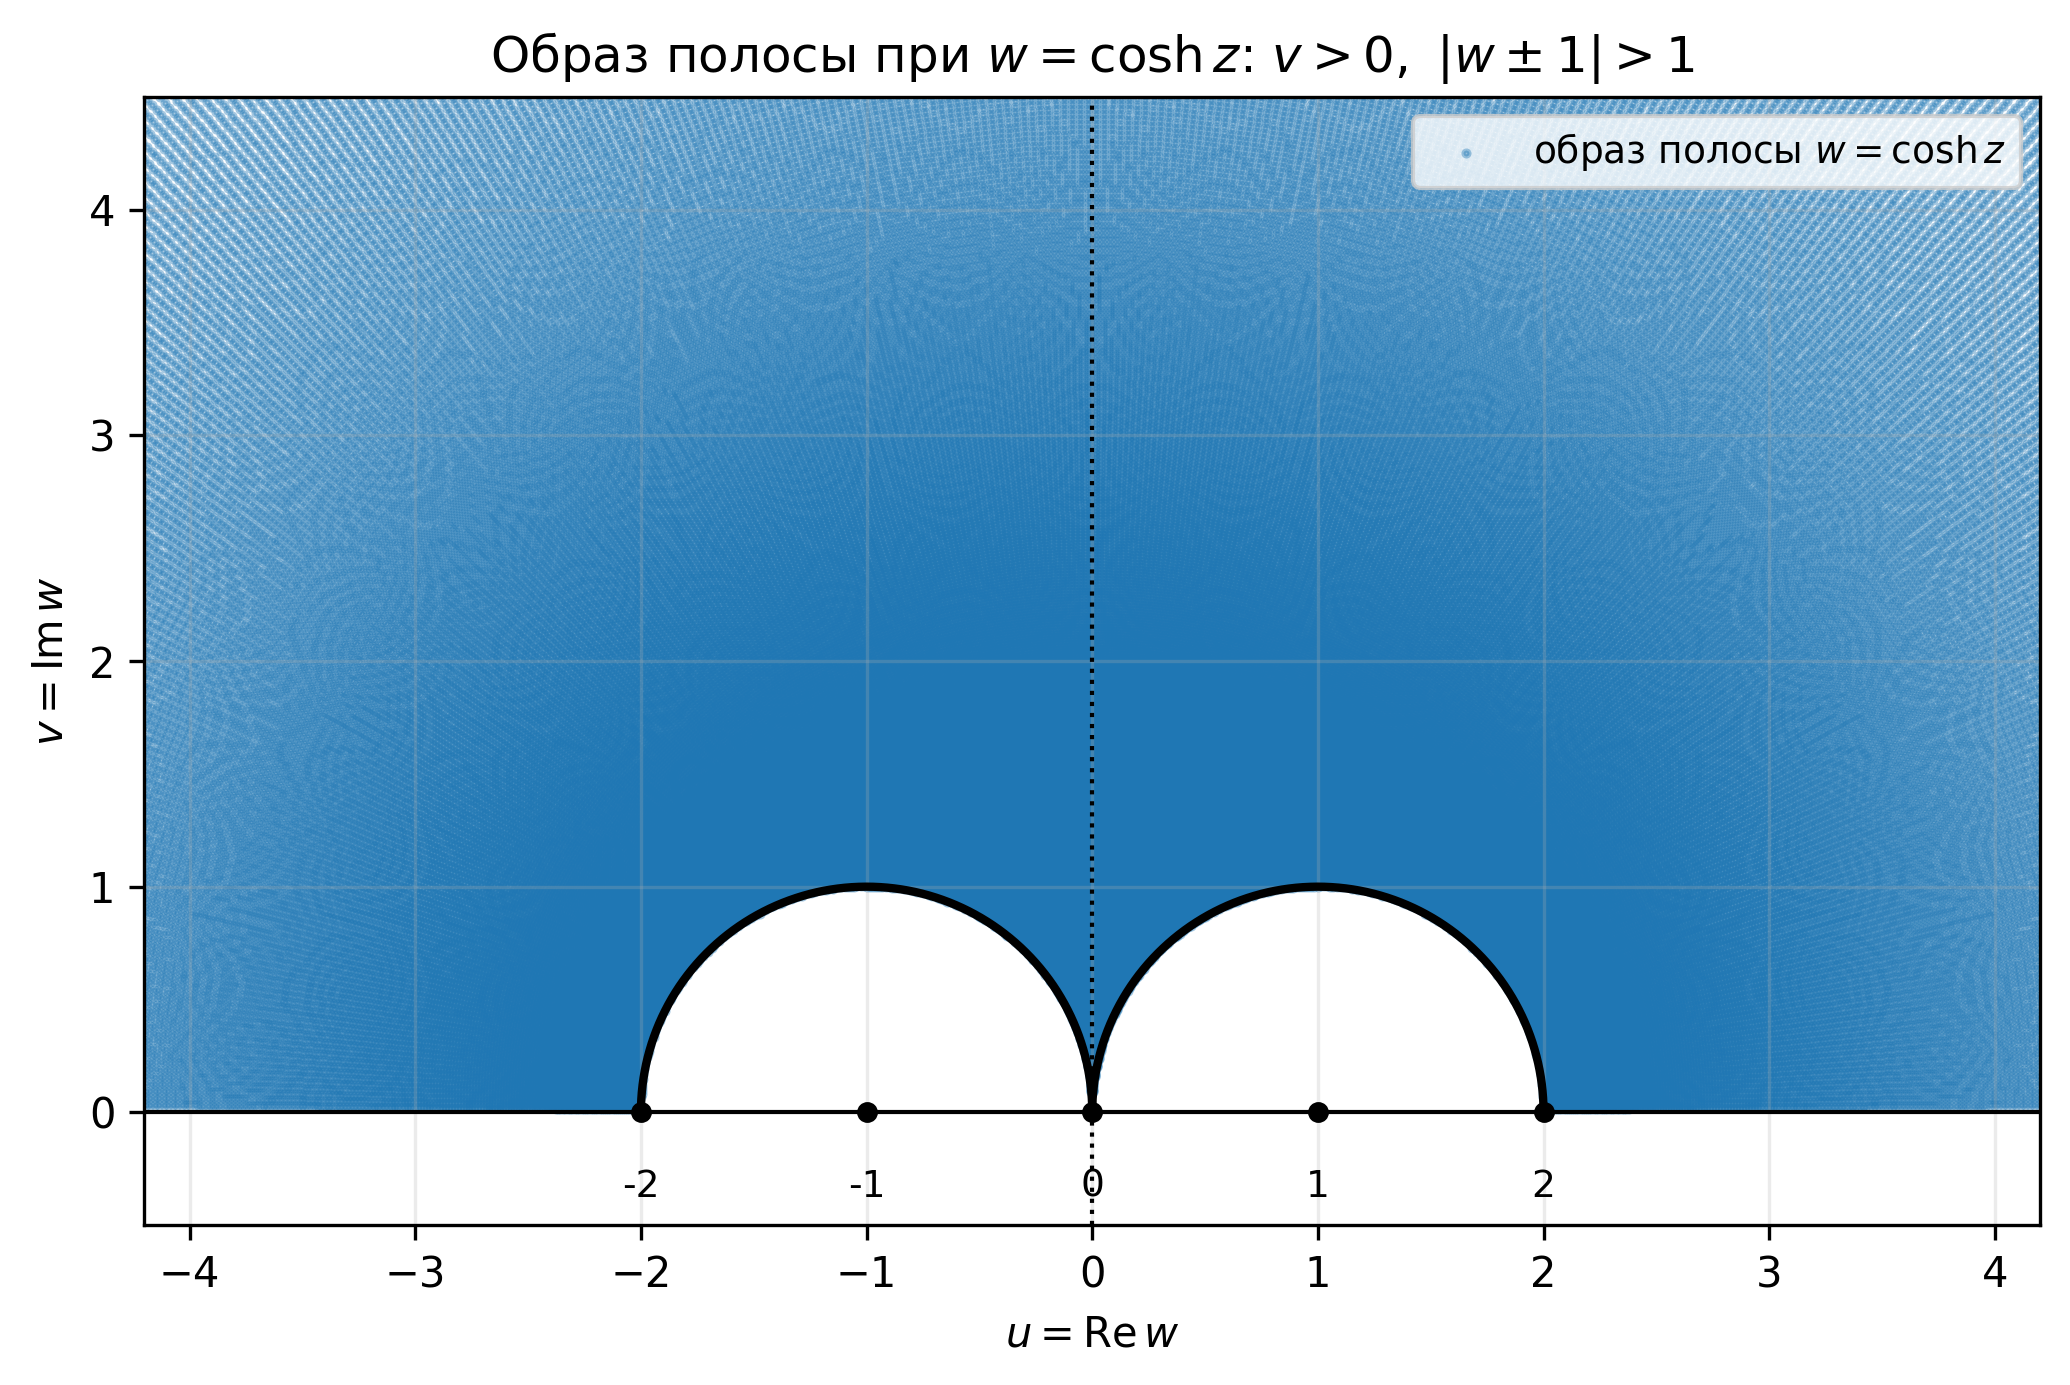
\includegraphics[width=1\linewidth]{cosh_strip_to_omega_w.png}
    \caption{Enter Caption}
    \label{fig:placeholder}
\end{figure}
\begin{figure}
    \centering
    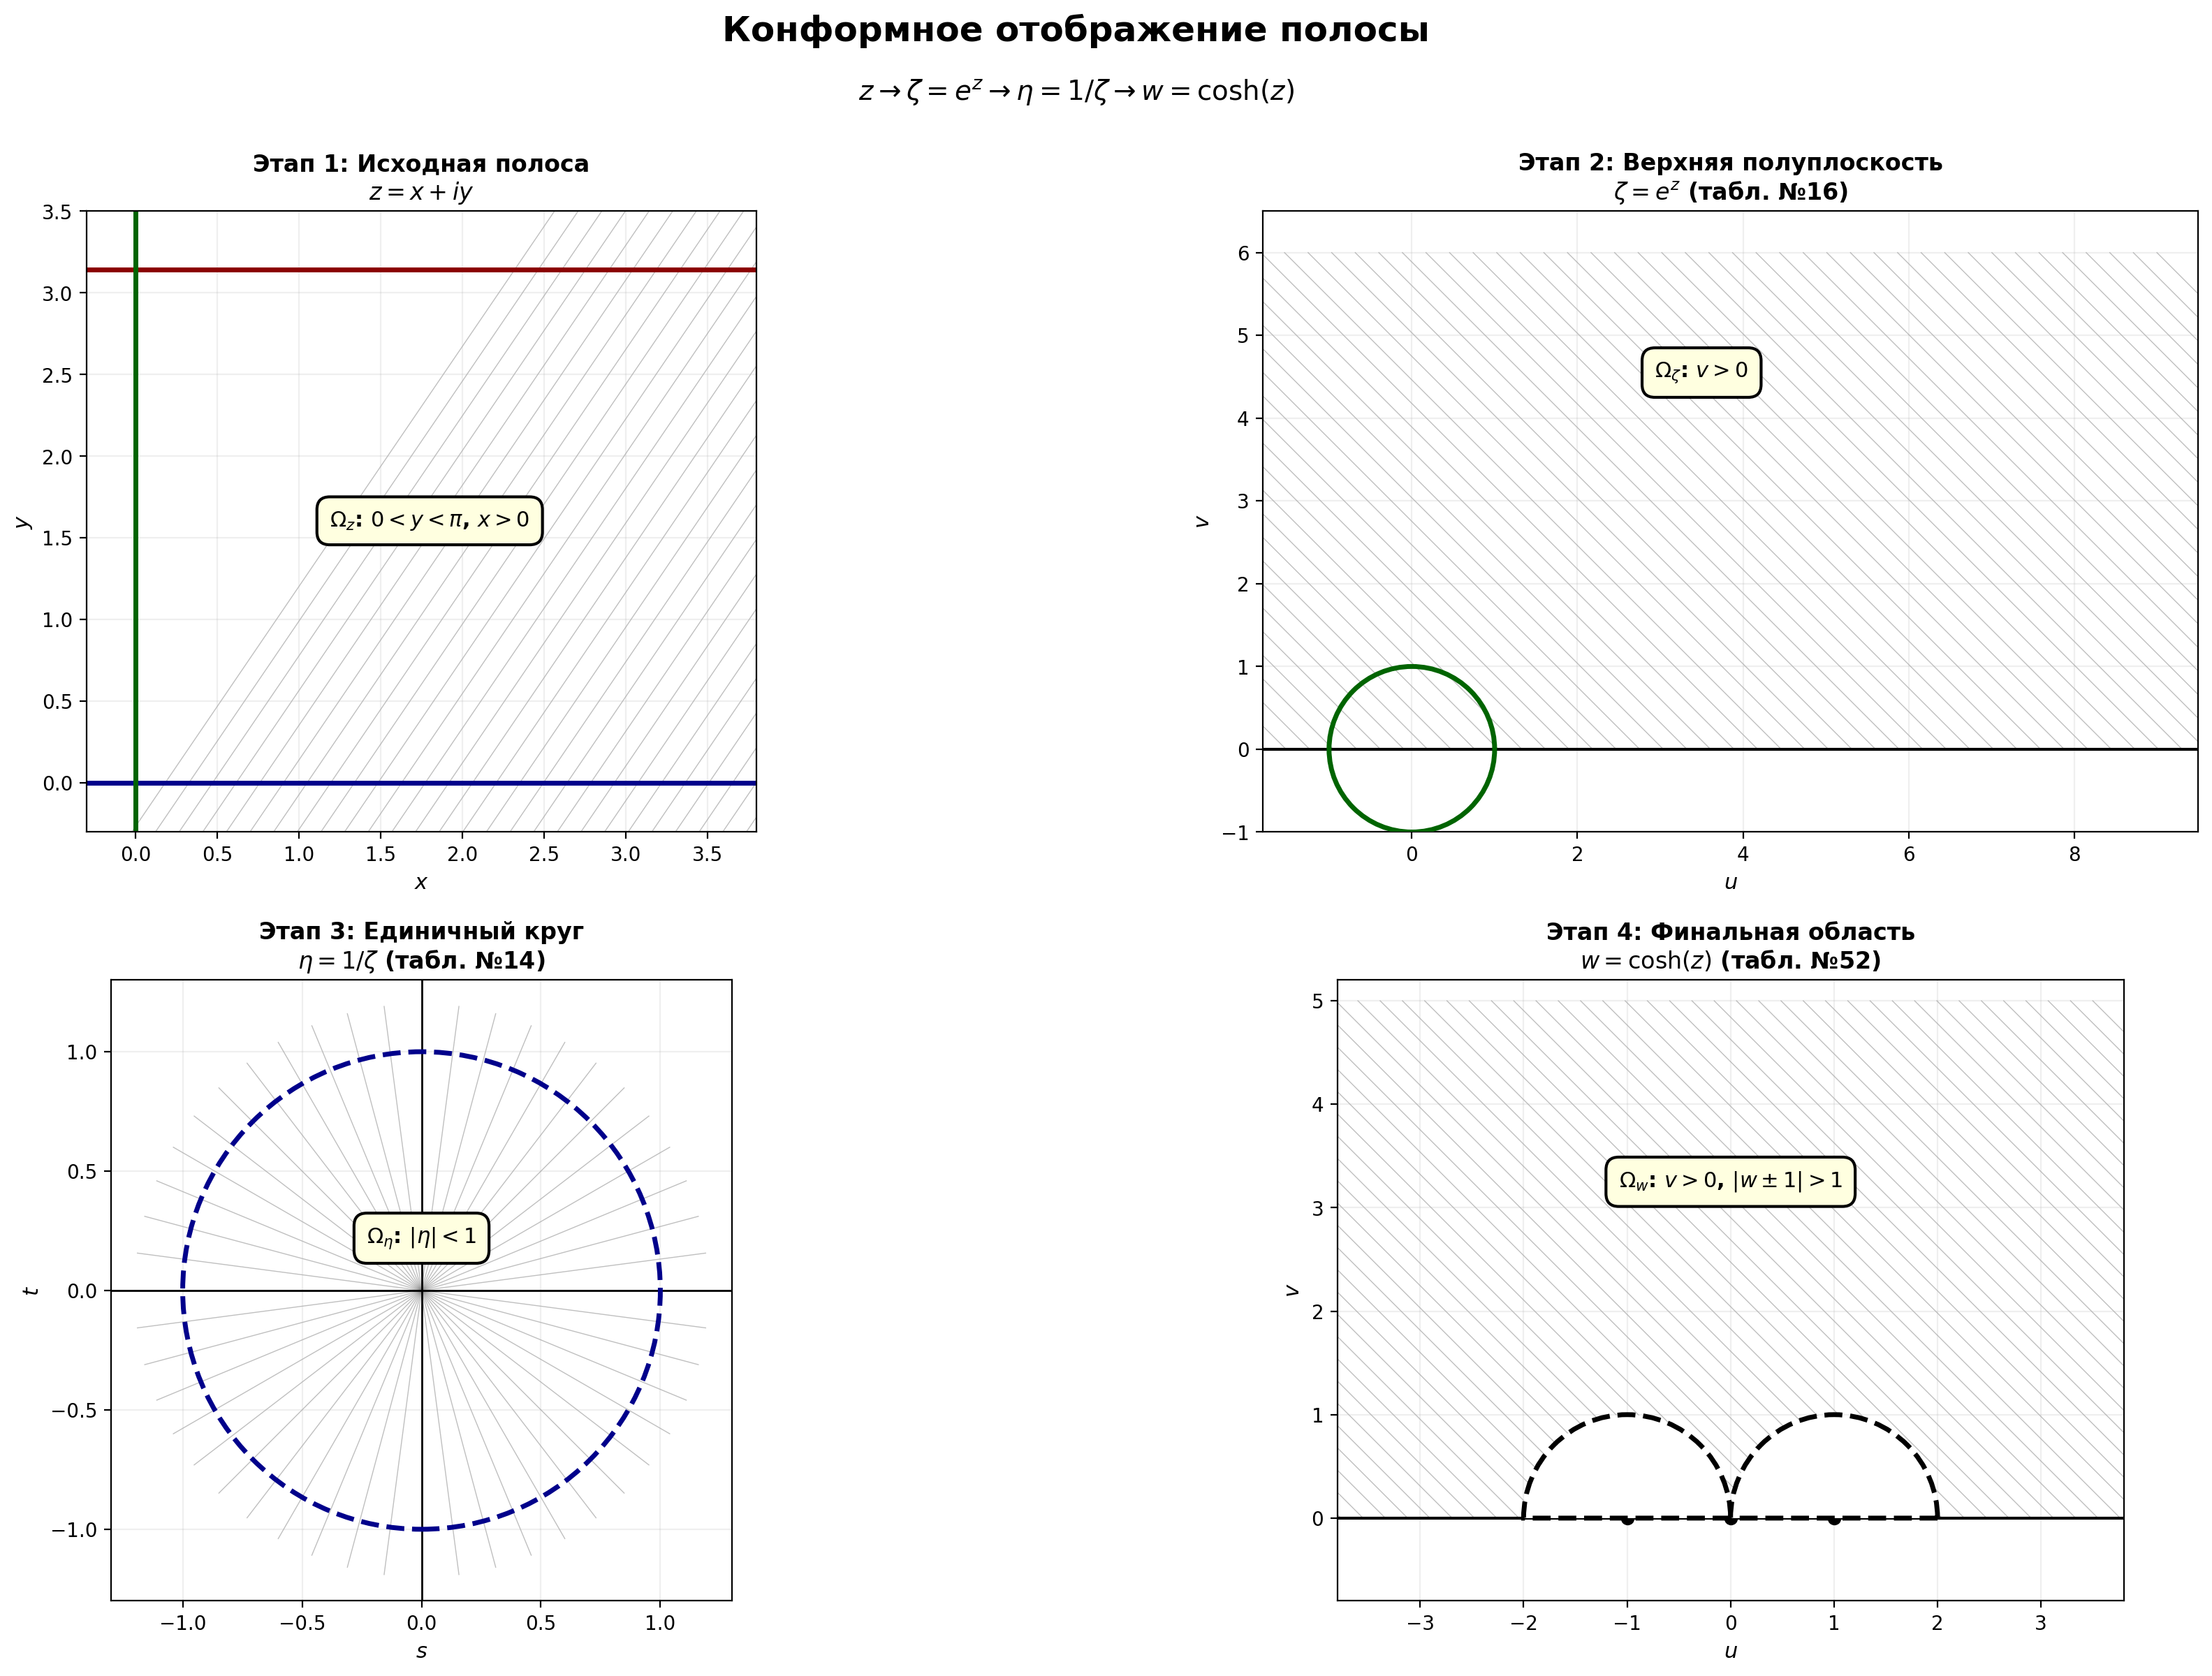
\includegraphics[width=1\linewidth]{image5.png}
    \caption{Все вместе}
    \label{fig:placeholder}
\end{figure}
\end{enumerate}

Каждый график содержит подробную аннотацию с формулами и описанием преобразования.

\end{document}